\chapter{Problem Solving: Architecture and Implementation Experience}
\label{ch:problem_solving}

\section{Chapter Scope}

This chapter explains how the problems described in Chapter~\ref{ch:problem_framing} are addressed.
The focus moves from the conceptual framing of the task to the operational design of the system, describing the architectural and implementation choices adopted to make the pipeline work.

The chapter is divided into two parts, the first part presents the architecture of the solution at a high level.
It mainly covers the streaming data engineering layer, including event sourcing, event streaming, and stream processing with Kafka and Flink.
It then describes the architectural choices used to construct the feature pipeline, feed the learning models, and compare their outputs.
The final part of the architectural overview introduces the models and their connection with the pipeline.
The goal is to explain how they are integrated into the overall system rather then discuss the learning algorithms in depth.

The second part zooms into the architecture and describes the implementation experience in more detail.
It explains the practical choices behind the implementation and how the problems introduced earlier were addressed at code and pipeline level.
This includes the choices that allowed the three decision paradigms to run, produce comparable outputs, and be evaluated under the same contracts.
The section also discusses the main algorithms, corrections, and implementation decisions that shaped the final system.

The quantitative results of the implementation and the comparison between paradigms are discussed in the following chapter.


\section{Architecture of the Solution}

This section describes the architecture of the implemented system. The emphasis is placed on the streaming data engineering part of the pipeline,
since this is the component that connects historical race data, live-like replay, stateful processing, and the artifacts later used for learning and evaluation.
The section first introduces the complete system view, and then discusses the main architectural blocks separately.

\subsection{Full Architecture Overview}

The system architecture is organized into three logical layers, as shown in Figure~\ref{fig:full_architecture}. The first layer is the \textit{Streaming Core Layer}.
It contains the components used to transform historical Formula 1 data into a replayable and processable stream. Historical data are first extracted from FastF1,
then converted into race events and replayed through Kafka topics. These topics are consumed by Flink, which processes the stream, maintains the race state, emits live
alerts, and persists JSONL artifacts used by the following stages. This layer is the operational base of the pipeline and is described in more detail in the next subsections.

The second layer is the \textit{Evaluation and Modelling Layer}. This layer starts from the artifacts produced by the streaming core and converts them into datasets,
feature matrices, and truth contracts. It includes the preparation of the Parquet training dataset, the definition of the prediction contracts, the evaluation of the
Flink Strategy Engine, and the training and evaluation of the learning-based approaches. After the models produce their scores or labels, the comparator and the threshold
frontier are used to make their outputs comparable under the same evaluation rules.

The final layer is the \textit{Delivery Layer}. Once the comparison artifacts have been produced, this layer is responsible for generating the material used to inspect
and report the results. It includes result analysis, figures, and audit checks over the produced data. The goal of this layer is
to make the outputs traceable and usable for the final experimental discussion presented in Chapter~\ref{ch:experimental_evaluation}.

\begin{figure}[htbp]
    \centering
    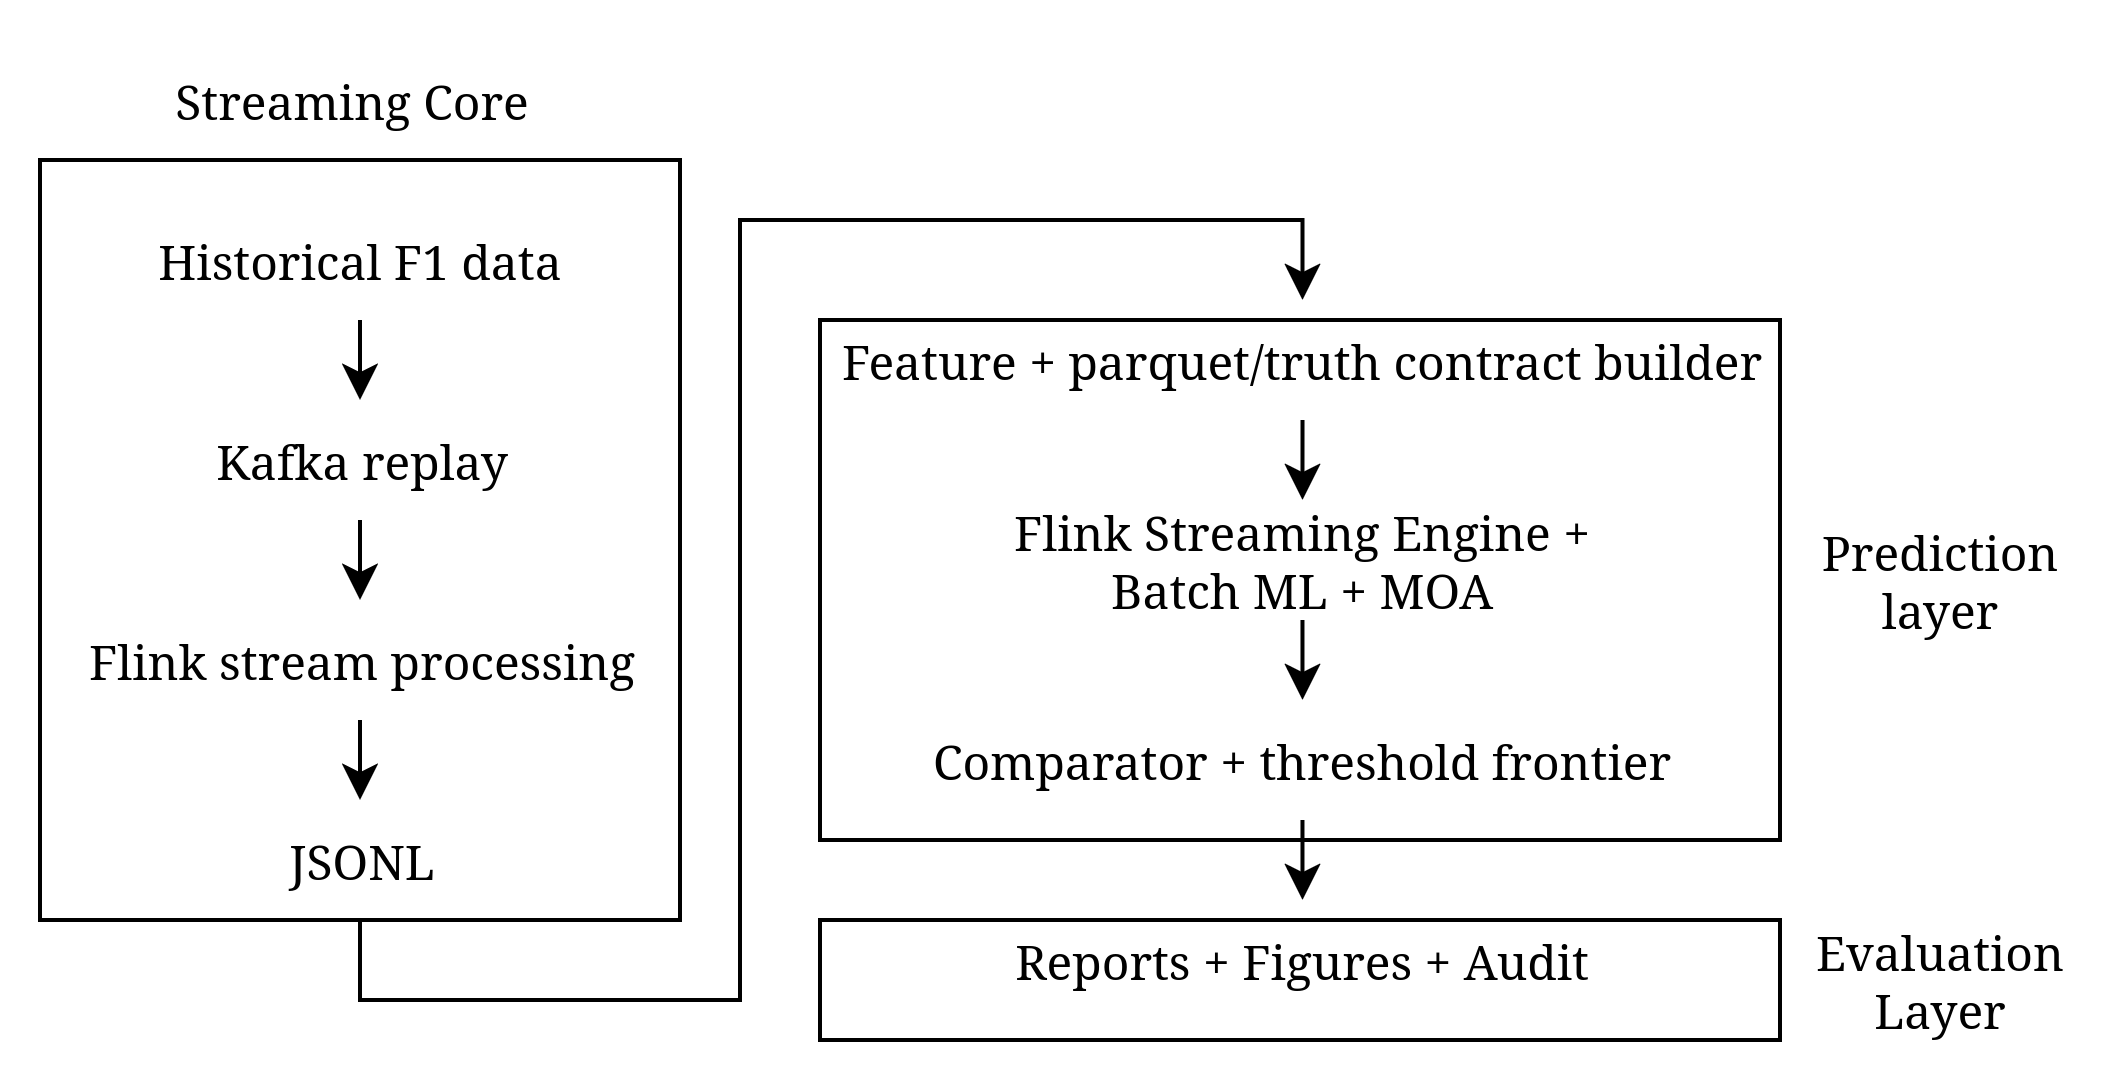
\includegraphics[width=0.75\textwidth]{Images/ch4/full_architecture.png}
    \caption{High-level architecture of the pipeline.}
    \label{fig:full_architecture}
\end{figure}


\subsection{Ingestion and Replay Architecture}

The pipeline starts in the Streaming Core Layer with the event sourcing stage. In this stage, a Python script retrieves historical race data from FastF1 and prepares the first
replayable representation of the race. The extracted data are cleaned, normalized, and enriched with the fields required by the replay and strategy pipeline. The details of
this preparation step are discussed later in Section~\ref{sec:historical_race_replay}. At this level, the relevant architectural point is that the race is prepared once and stored as a Parquet artifact,
so that the same session can be replayed multiple times without repeating the extraction process.

The replay stage is handled by a second Python script. This script reads the prepared Parquet data and publishes the race events to Kafka, race by race. The replay follows the
original event time of the race, so the order of the streamed observations reflects the natural progression of the session rather than the speed at which the experiment is executed.
This separation between preparation and replay makes the stream controllable: the same race snapshot can be replayed again for debugging, regeneration of artifacts, or comparison
between different downstream configurations.

Kafka organizes the replay into three topics with different granularities: telemetry, laps, and track status. The telemetry topic contains the highest-frequency stream and describes
continuous car-level signals. The laps topic emits one event per driver and completed lap, carrying more aggregated information such as lap time, position, tyre life, stint information,
and pit-related markers. The track-status topic is sparser and represents global race conditions, such as yellow flags, virtual safety cars, safety cars, and similar session-level
events. Keeping these streams separated allows the processing layer to combine high-frequency car behaviour, lap-level race state, and global race context when needed.

The ingestion and replay architecture therefore provides a reproducible entry point for the whole system. Historical data are fetched, prepared, stored once, and then streamed
through Kafka in a consistent and analyzable form. This supports the main experimental requirement of the pipeline: the same historical race can be replayed several times while
preserving the same input evidence for the following Flink, learning, and evaluation stages.

\begin{figure}[htbp]
    \centering
    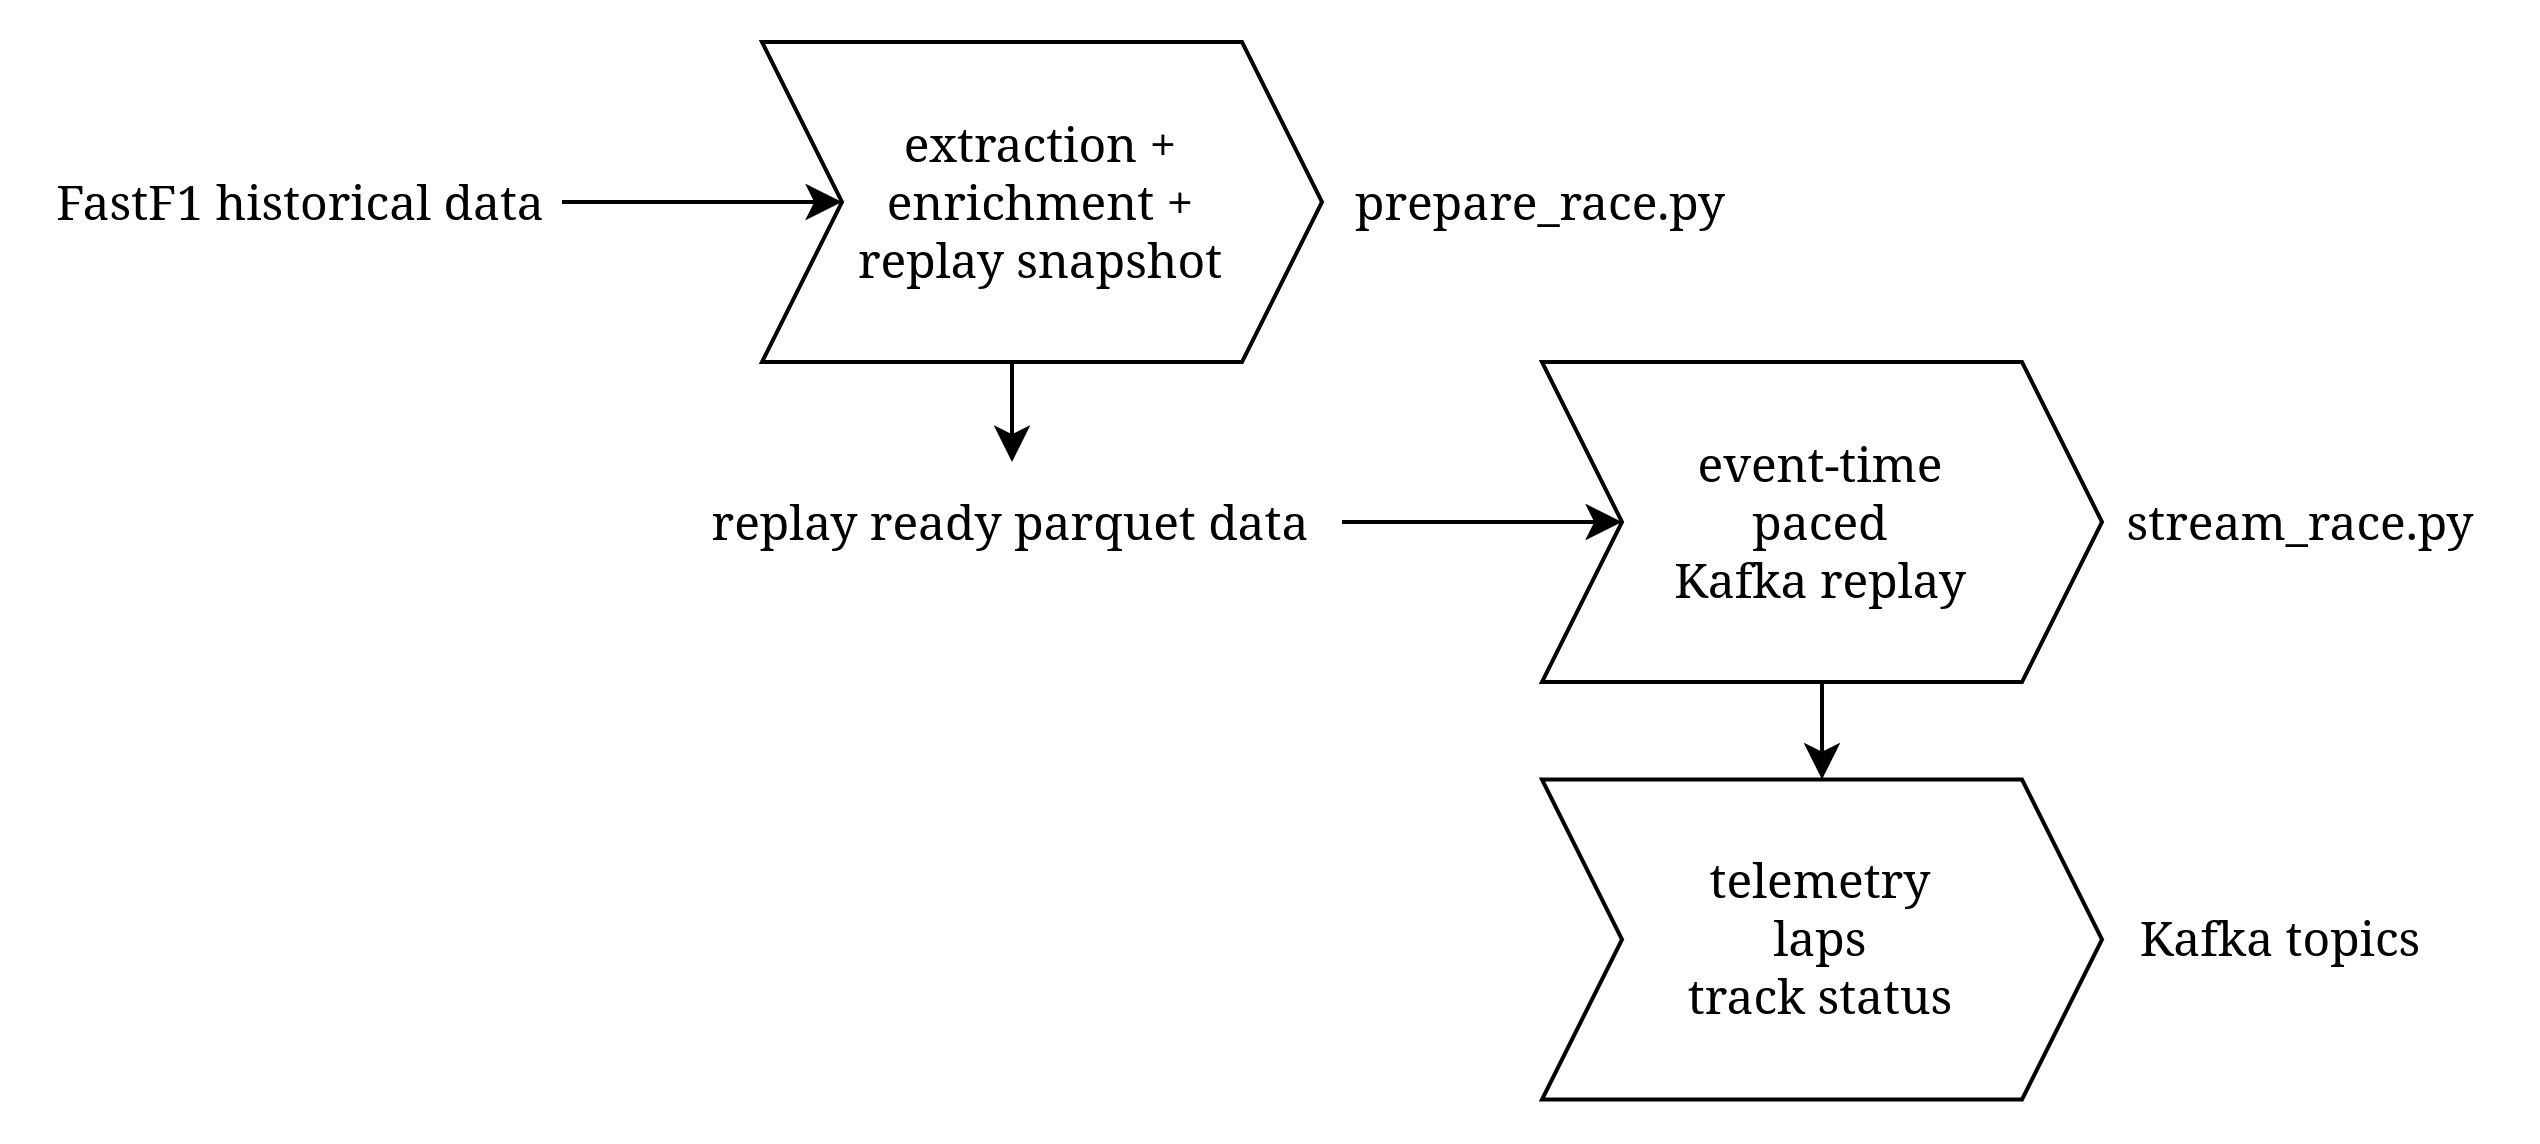
\includegraphics[width=0.75\textwidth]{Images/ch4/ingestion&replay.png}
    \caption{Ingestion and replay architecture. Historical race data are extracted and stored once as replay-ready Parquet artifacts, then replayed through Kafka as telemetry,
        lap, and track-status streams.}
    \label{fig:ingestion_replay_architecture}
\end{figure}


\subsection{Flink Stream-Processing Architecture}

After the replay stage publishes the race topics to Kafka, Flink consumes them and becomes the main stream-processing component of the system. Its role is to transform the 
incoming race streams into race-aware strategy signals and persistent artifacts. The processing follows event time, so the state of the race is updated according to the original 
race chronology rather than according to the execution speed of the replay.

At this architectural level, the relevant point is that Flink maintains the evolving race context needed by the downstream components. Event-time processing is used to order 
race observations, state is used to remember information such as track status, gaps, tyre history, and previous driver context, while windows group events around race and lap-level 
situations. On top of this stateful layer, strategy operators compute the main intermediate signals used by the system, including rival context, tyre drops, drop zones, pit evaluations, 
and pit suggestions. The detailed logic used to construct these signals is described later in Sections~\ref{sec:race_context_building} and~\ref{sec:pit_suggestion_and_classification}.

The output of this stage has two forms. Live alerts are sent back to Kafka so that they can be consumed during the replay, while JSONL artifacts are persisted to the data lake 
and reused by the feature, learning, and evaluation stages. Flink therefore acts as the boundary between live-like stream processing and reproducible downstream analysis.

\begin{figure}[htbp]
    \centering
    
\includegraphics[width=0.75\textwidth]{Images/ch4/flink.png}
    \caption{Flink stream-processing architecture. Kafka topics are consumed with event-time semantics, enriched through stateful race context, and transformed into strategy signals, live alerts, and persisted JSONL artifacts.}
    \label{fig:flink_stream_processing_architecture}
\end{figure}

\subsection{Data Lake and Feature Architecture}

After the Flink processing stage, the stream outputs are persisted in the data lake as JSONL artifacts. This storage step defines the boundary between the live-like streaming part of 
the system and the reproducible learning and evaluation part. The same race replay can generate live alerts during execution, but the downstream models and comparators require 
stable files that can be inspected, joined, and reused without running the stream again.

The data lake contains several families of artifacts. The pit timing and pit evaluation outputs describe the truth side of the problem, since they record real pit events and the 
post-pit outcome labels. The drop-zone and tyre-degradation outputs describe additional race context generated by the stream-processing logic. The pit suggestion stream stores the 
rule-based decisions emitted by the Flink Strategy Engine, while the ML feature stream stores the per-driver, per-lap rows used by the learning pipeline.

Dataset preparation starts from these JSONL files and converts them into a Parquet training dataset. This step performs deduplication, joins the different stream outputs, removes 
fields that would introduce target leakage, and builds the horizon-based labels used by the prediction contracts. The resulting dataset is therefore 
a structured representation of the same stream artifacts produced by Flink.

Dataset preparation also defines the feature contract used by the learning branches.
This step applies feature filtering and selected feature transformations, fields that would expose target information or shortcut information are removed, while some 
raw race quantities are converted into more comparable representations. For example, race progress and driver pace can be expressed as percentage features, so 
that the learner receives values that are less tied to a specific circuit length or absolute lap time scale. The detailed motivation for source-year removal and the percent 
feature profile is discussed later in Section~\ref{sec:source_year_removal} and Section~\ref{sec:percent_feature_profile}.

This architecture keeps the feature construction step traceable. The learning models do not access the original race outcome directly; they receive a filtered and aligned dataset 
derived from the persisted stream outputs. In this way, the data lake acts as the contract boundary between streaming engineering, Batch and MOA learning, and the final evaluation 
protocol.

\begin{figure}[htbp]
    \centering
    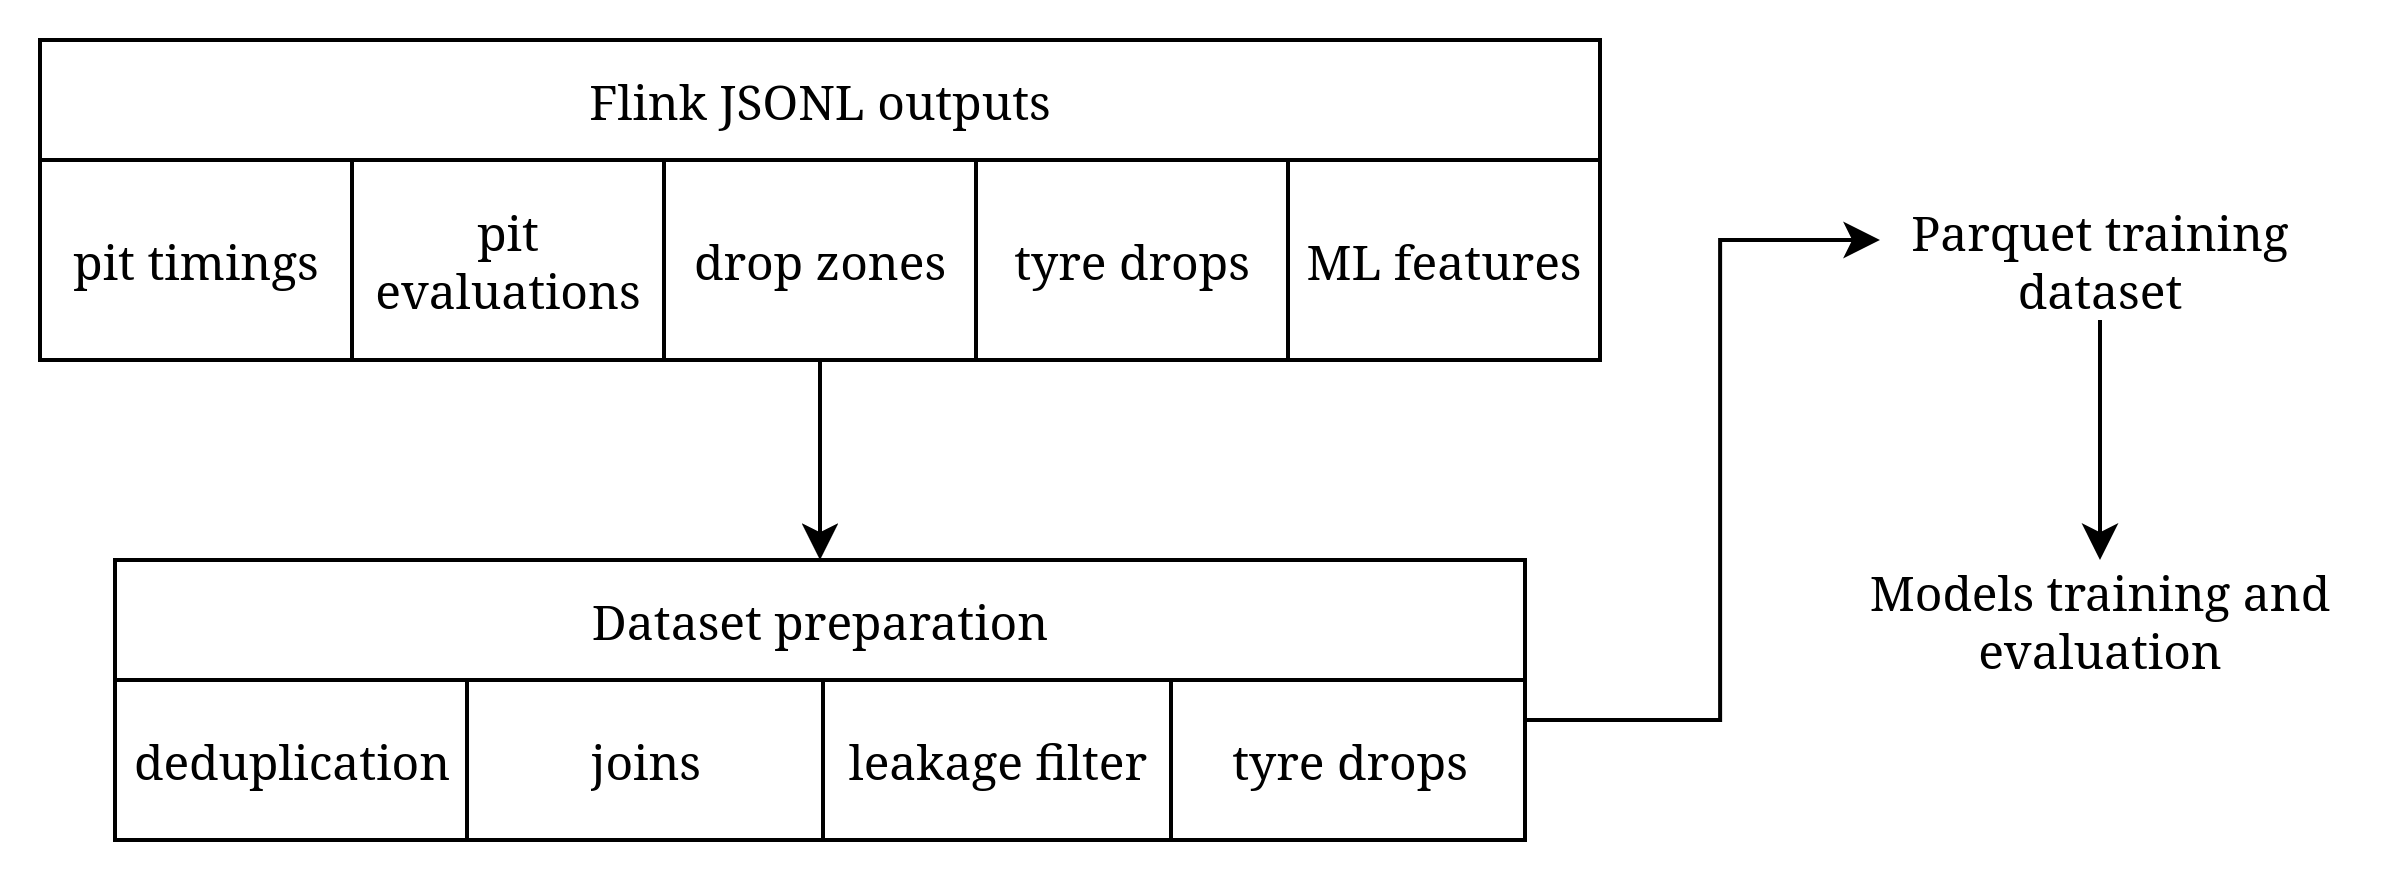
\includegraphics[width=0.75\textwidth]{Images/ch4/dataset_prep.png}
    \caption{Data lake and feature architecture.}
    \label{fig:data_lake_feature_architecture}
\end{figure}

\subsection{Truth and Comparator Architecture}

After the data lake boundary has been defined, the next architectural step is to define how predictions are compared with the truth. This layer is needed because the three decision 
systems produce different types of output. Before these outputs can be compared, they have to be converted into positive calls and matched against the same prediction contracts.

The two main contracts are \texttt{pit\_any\_h2} and \texttt{pit\_success\_h2}. In the \texttt{pit\_any\_h2} contract, a positive prediction at lap $k$ is correct if an eligible 
pit stop occurs in the following two laps, that is, in the future window $[k+1, k+2]$. This contract represents the pit timing problem. In the \texttt{pit\_success\_h2} contract, 
a positive prediction is correct only if an eligible pit stop occurs in the same window and that stop is later classified as successful by the post-pit evaluation pipeline. 
This second contract is stricter, because the system must predict both the timing of the pit and the fact that the pit will correspond to a positive strategic outcome.

The truth used for training and comparison comes from real pit events and from their classification after 
the stop has occurred. The comparator uses this truth layer to evaluate the calls produced by Flink, Batch XGBoost, and MOA with the same horizon and the same eligible event universe.


\subsection{Model Architecture}

The final architectural block concerns the way the three decision systems are connected to the common evaluation pipeline. At this point, 
the truth contracts and the feature artifacts have already been defined. The remaining issue is that the systems do not produce the same type of output, even though they 
must be evaluated under the same contracts.

The Flink Strategy Engine emits rule-based recommendation labels, such as \texttt{MONITOR}, \texttt{GOOD\_PIT}, and \texttt{PIT\_NOW}. For the operational comparison, 
\texttt{PIT\_NOW} is treated as a positive pit call. Batch XGBoost instead produces out-of-fold probability scores, while the MOA Online Learner produces vote-based 
scores during prequential evaluation. For both learning-based systems, positive calls are obtained by applying a selected threshold to the score.

The model architecture therefore hides the difference in output format behind a common decision representation. After conversion, each system produces the same logical 
object: a positive call associated with a race, a driver, and a lap. The comparator can then match these calls against the same future horizon truth contracts. 
In this way, the three systems keep their different decision mechanisms, while the final scoring remains shared.


\section{Implementation Experience}

% Maps to presentation slides 27--38.
%
% This section is more practical than the architecture section.
% It explains how the architecture was progressively turned into the thesis experiment.

\subsection{Historical Race Replay}
\label{sec:historical_race_replay}

% Slide 27.
%
% Goal:
% Describe implementation phase 1.
%
% Content to cover:
% \begin{itemize}
%     \item FastF1 loads a race session;
%     \item telemetry, laps, and track status are extracted;
%     \item events are enriched with gaps, weather, and pit-loss information;
%     \item events are ordered by event time;
%     \item the prepared race is saved as Parquet;
%     \item the saved race can then be streamed to Kafka with a replay speed and optional start lap.
% \end{itemize}
%
% Main phrase:
% freeze the race once, then replay it many times as a controlled live-like stream.

\subsection{Persisted Stream Outputs}
% Slide 28.
%
% Goal:
% Describe implementation phase 2.
%
% Content to cover:
% \begin{itemize}
%     \item Flink converts race streams into persisted strategy artifacts;
%     \item truth artifacts include \texttt{pit\_timings} and \texttt{pit\_evals};
%     \item race-context artifacts include \texttt{drop\_zones}, \texttt{tire\_drops}, and \texttt{lift\_coast};
%     \item decision-stream artifacts include \texttt{pit\_suggestions};
%     \item ML-contract artifacts include \texttt{ml\_features};
%     \item these JSONL outputs connect live stream processing to reproducible Batch/MOA evaluation.
% \end{itemize}

\subsection{Race Context Building in Flink}
\label{sec:race_context_building}
% Slide 29.
%
% Goal:
% Explain which context metrics are built in the stream.
%
% Content to cover:
% \begin{itemize}
%     \item gaps and rivals are built by ordering drivers by lap position and computing local gap context;
%     \item tyre degradation compares current lap pace against stint-best pace;
%     \item drop zone estimates where the car would rejoin if it pitted;
%     \item track status is broadcast into the strategy logic;
%     \item these metrics feed both strategy alerts and ML feature rows.
% \end{itemize}
%
% Optional formulas from slide:
% \begin{itemize}
%     \item \texttt{paceRatio = (lapTime - stintBest) / stintBest}
%     \item tyre drop condition based on \texttt{lapTime > stintBest * (1 + theta)}
%     \item drop-zone computation based on accumulated gaps and pit loss
% \end{itemize}

\subsection{Pit Suggestion and Pit Classification Logic}
\label{sec:pit_suggestion_and_classification}
% Slide 30.
%
% Goal:
% Explain why the implementation keeps two paths separate.
%
% Content to cover:
% \begin{itemize}
%     \item pit suggestion happens before the pit;
%     \item pit classification happens after a real pit;
%     \item suggestion labels include \texttt{MONITOR}, \texttt{GOOD\_PIT}, \texttt{PIT\_NOW}, and \texttt{LOST\_CHANCE};
%     \item pit classification produces success, failure, or unresolved labels;
%     \item the pit suggestion score combines pace, track status, traffic, strategy penalty, urgency, timing pressure, end-of-race penalty, competitive pressure, and uncertainty penalty;
%     \item post-pit outcome classification compares post-pit and pre-pit gap conditions.
% \end{itemize}



\subsection{Addressing Invalid Data and Leakage Risks}

% Slide 31.
%
% Goal:
% Explain the corrections that were needed to turn the working pipeline into a fair thesis experiment.
%
% Content to cover:
% \begin{itemize}
%     \item different race/event universes required a shared canonical truth universe;
%     \item past/future contamination required chronological or race-wise evaluation;
%     \item target leakage required removing target, truth, matched-pit, and eligibility fields;
%     \item ambiguous truth definitions required explicit truth lenses;
%     \item shortcut features required removing \texttt{\_source\_year}.
% \end{itemize}


\subsection{Flink Strategy Engine Variants}

% Slide 32.
%
% Goal:
% Explain implementation phase 4.
%
% Content to cover:
% \begin{itemize}
%     \item the rule-based baseline was tuned before the final Batch/MOA comparison;
%     \item the Strict version was conservative and disabled promotion mechanisms;
%     \item the Rival-pressure version increased reach by enabling rival-pressure promotion;
%     \item the Guarded rival-pressure version kept rival pressure but added guards against noisy promotions;
%     \item the guarded version was frozen as the final Flink Strategy Engine version.
% \end{itemize}


\subsection{Batch ML Pipeline}

% Slide 33.
%
% Goal:
% Explain implementation phase 5.
%
% Content to cover:
% \begin{itemize}
%     \item Batch ML is expressed as race-sequential out-of-fold evaluation;
%     \item for each held-out race, training uses previous races;
%     \item XGBoost predicts scores on the held-out race;
%     \item out-of-fold scores are appended into a table;
%     \item thresholds are swept on OOF scores;
%     \item feature filtering removes metadata, target fields, truth fields, and matched-pit fields;
%     \item XGBoost is used as a binary logistic classifier with \texttt{aucpr};
%     \item calibration is treated as probability-quality diagnostic, not as a guarantee.
% \end{itemize}


\subsection{Source-Year Removal}
\label{sec:source_year_removal}
% Slide 34.
%
% Goal:
% Explain implementation phase 6.
%
% Content to cover:
% \begin{itemize}
%     \item the first dataset contained \texttt{source\_year};
%     \item \texttt{source\_year} could encode season-level shortcuts;
%     \item SHAP exposed it as an important feature;
%     \item after removal, feature importance shifted toward race-state features such as tyre life, race progress, and pace signals.
% \end{itemize}


\subsection{Percent Feature Profile}
\label{sec:percent_feature_profile}
% Slide 35.
%
% Goal:
% Explain implementation phase 7.
%
% Content to cover:
% \begin{itemize}
%     \item some raw race values were transformed into race-relative signals;
%     \item \texttt{race\_progress\_pct} describes where the car is in the race;
%     \item \texttt{lapTime\_vs\_driver\_prev\_mean\_pct} describes current pace relative to previous driver pace;
%     \item conservative exclusions remove team and rainfall from this profile;
%     \item Percent is an engineered profile partly motivated by Batch explainability;
%     \item No-Year remains the cleaner neutral baseline;
%     \item the same feature contract is exported to both Batch and MOA.
% \end{itemize}


\subsection{MOA Export}

% Slide 36.
%
% Goal:
% Explain implementation phase 8.
%
% Content to cover:
% \begin{itemize}
%     \item MOA requires a different input format from XGBoost;
%     \item the export step converts the Batch feature matrix into a MOA-compatible stream dataset;
%     \item the matrix contract is preserved;
%     \item exported elements include CSV, ARFF, schema JSON, and binary target labels;
%     \item Batch and MOA differ in learning paradigm, not in input semantics.
% \end{itemize}


\subsection{MOA Prequential Evaluation}

% Slide 37.
%
% Goal:
% Explain implementation phase 9.
%
% Content to cover:
% \begin{itemize}
%     \item streaming ML is evaluated in stream order;
%     \item for each instance, the learner predicts first;
%     \item the prediction and vote information are logged;
%     \item the learner then trains on the same instance;
%     \item this preserves the test-then-train order;
%     \item the current prediction cannot use future rows.
% \end{itemize}


\subsection{MOA Vote Logger}

% Slide 38.
%
% Goal:
% Explain implementation phase 10.
%
% Content to cover:
% \begin{itemize}
%     \item initial MOA output was mostly hard 0/1 labels;
%     \item hard labels made threshold sweeps weak;
%     \item the custom logger records class votes before training on the instance;
%     \item \texttt{positive\_score = vote\_1 / (vote\_0 + vote\_1)};
%     \item the learning protocol remains unchanged;
%     \item continuous vote scores enable AP, PR curves, and threshold-frontier diagnostics.
% \end{itemize}


\section{Chapter Summary}

% Briefly close the chapter:
% the architecture creates a reproducible path from historical races to stream artifacts,
% and the implementation experience shows how the Flink, Batch, and MOA branches were made
% comparable under the same contracts.
% The quantitative comparison is left to Chapter~\ref{ch:experimental_evaluation}.